\section{Analysis}
\label{sec:analysis}

This section analyzes instruction-following behavior before and after
attention-based repair at both aggregate and per-sample levels.
While Section~\ref{sec:experiments} focuses on representative qualitative
case studies, the analysis here aims to identify broader quantitative trends
and internal patterns that help explain the observed recovery behavior.

\subsection{Aggregate Instruction-Following Recovery}

\begin{figure}[t]
  \centering
  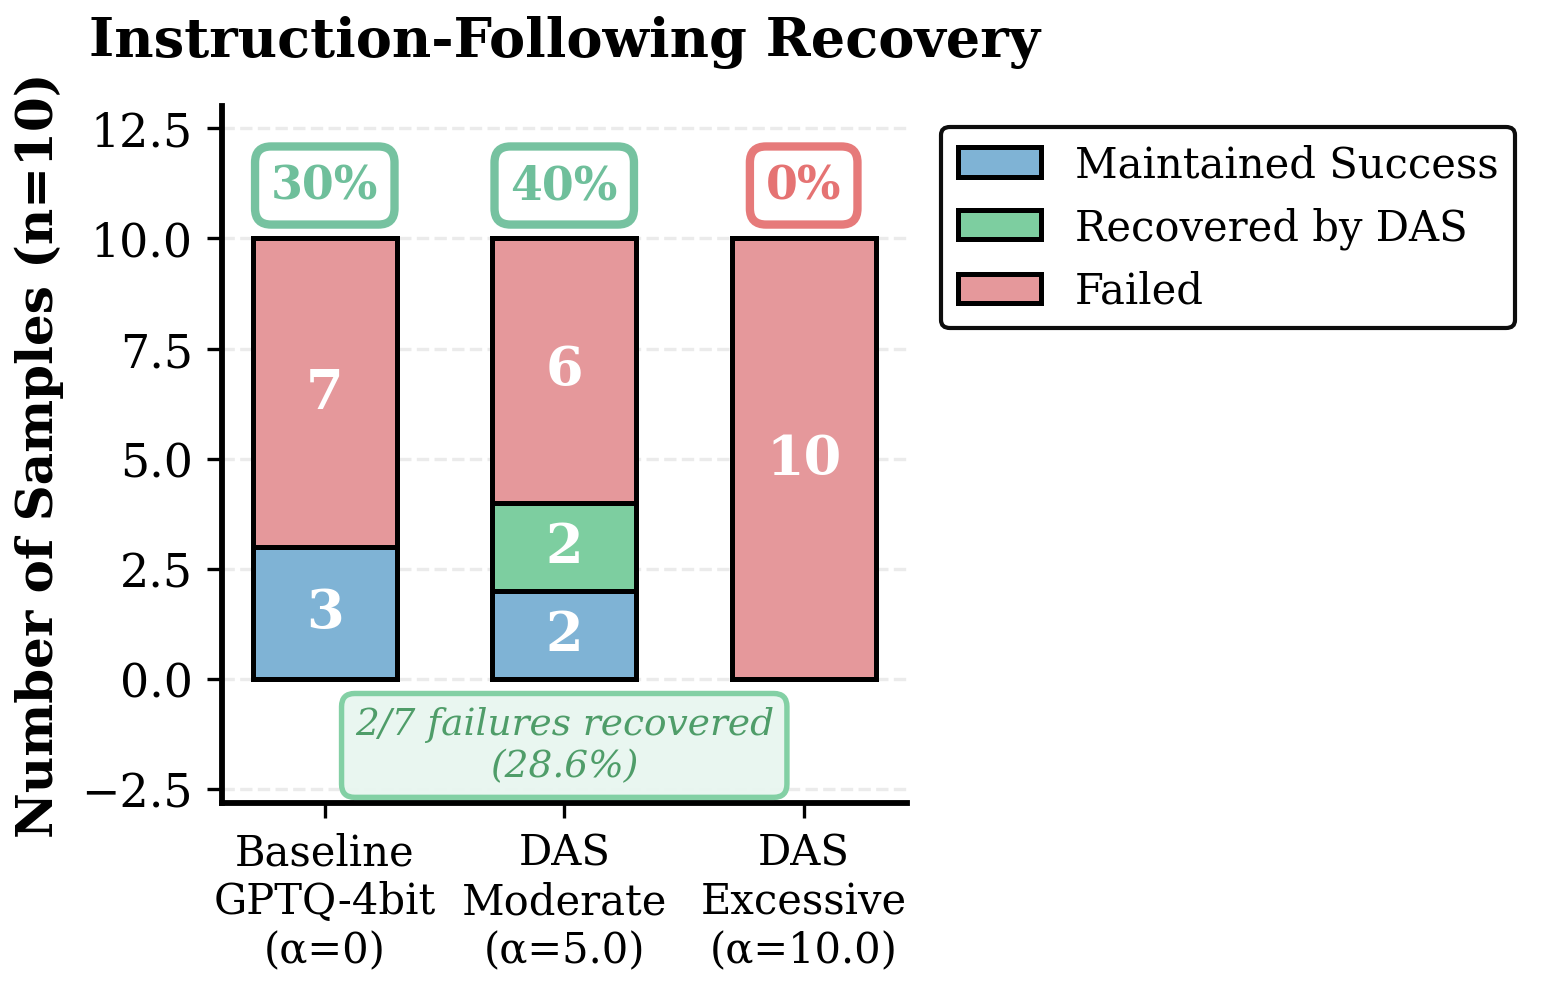
\includegraphics[width=\columnwidth]{figures/figure4.png}
  \caption{Aggregate and per-sample instruction-following outcomes under different
  stimulation strengths.
  The left panel summarizes recovery statistics across samples.
  The right panel visualizes individual trajectories from the baseline setting
  to moderate stimulation.}
  \label{fig:alpha}
\end{figure}

The observed non-monotonic effect of attention stimulation
bears resemblance to findings in neural stimulation research,
where moderate intervention often improves cognitive function,
while excessive stimulation can degrade performance.
In modern neuroscience and clinical studies,
brain stimulation techniques such as transcranial electrical stimulation
have been shown to exhibit dose-dependent effects,
with optimal stimulation levels varying across tasks and individuals
\citep{dayan2001theoretical,buzsaki2006rhythms,miniussi2013tdcs}.

Figure~\ref{fig:alpha} summarizes instruction-following outcomes before and after
repair across multiple samples.
At the baseline setting $\alpha = 0.0$, most samples fail to satisfy instruction
constraints.
With moderate stimulation at $\alpha = 5.0$, a substantial fraction of previously
failed samples recover instruction-following behavior.
In contrast, excessive stimulation at $\alpha = 10.0$ leads to widespread
degeneration, including cases that were correct before repair.

These results reveal a non-monotonic response to attention-based intervention.
Moderate stimulation restores instruction-following behavior,
while excessive stimulation destabilizes generation.
Such non-linear effects are consistent with observations from neural intervention
studies, where moderate perturbations restore functional activity while stronger
perturbations impair performance
\citep{dayan2001theoretical,buzsaki2006rhythms}.

\subsection{Per-Sample Trajectories and Variability}

Beyond aggregate trends, Figure~\ref{fig:alpha} also illustrates per-sample
trajectories from the baseline setting to moderate stimulation.
Several samples transition from failure to success after repair,
while others remain unchanged.
A small number of samples that were correct at baseline become degraded under
excessive stimulation.

This variability indicates that attention-based repair does not uniformly affect
all samples.
Instead, recovery is localized to a subset of failure cases.
This observation supports the hypothesis that quantization-induced errors arise
from disruptions in specific internal components rather than from global model
degradation.
Similar heterogeneity has been reported in prior mechanistic analyses of
transformer models
\citep{olah2020zoom,elhage2021mechanistic,nanda2023progress}.

\subsection{Attention-Level Patterns Under Repair}

\begin{figure}[t!]
  \centering
  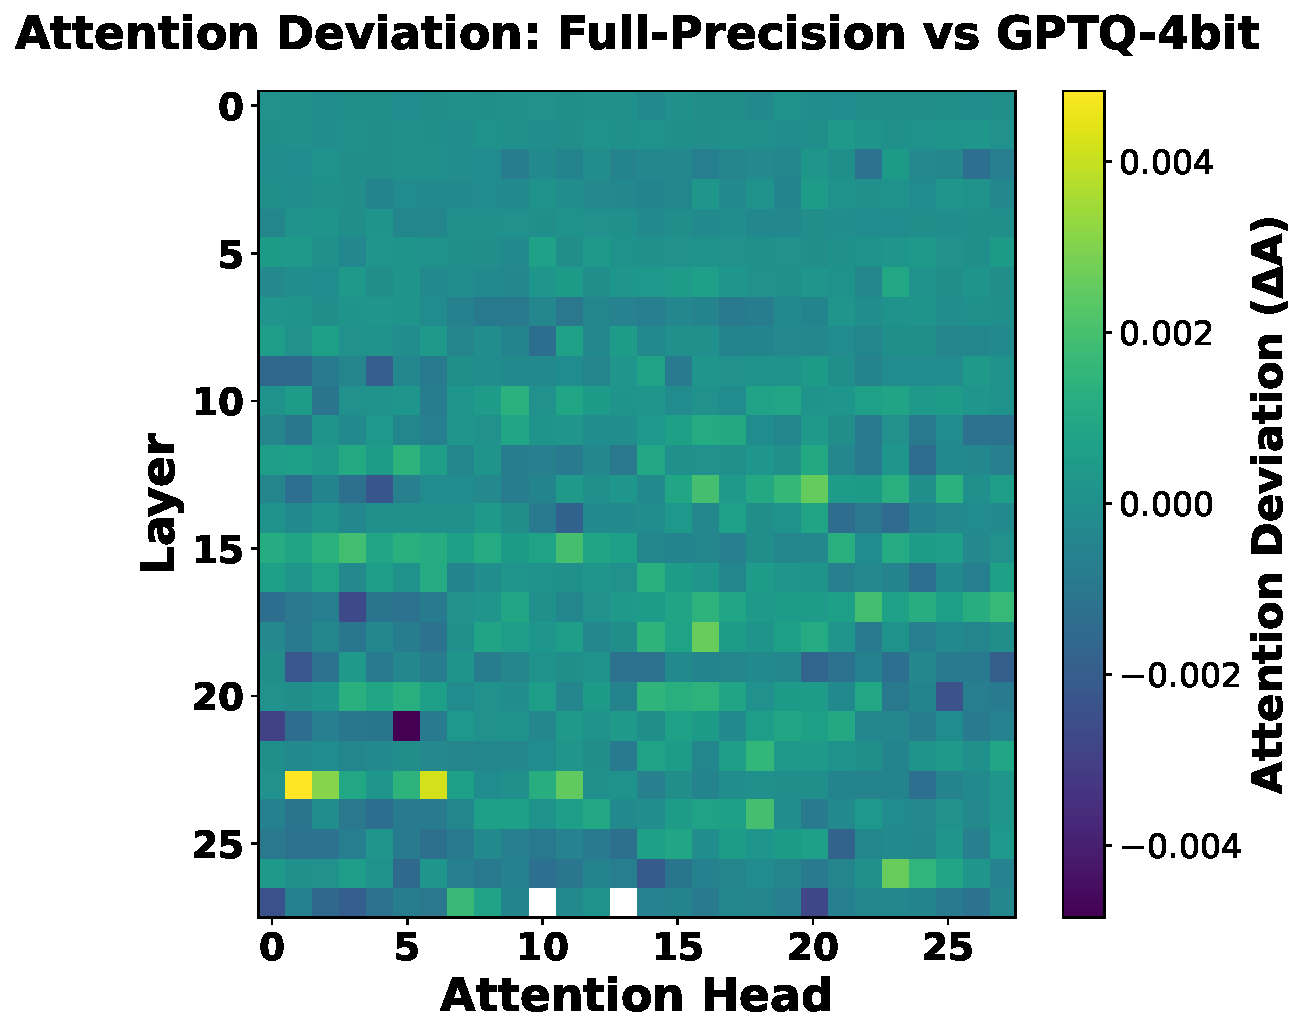
\includegraphics[width=\columnwidth]{figures/figure5_heatmap1.pdf}
  \caption{Attention deviation heatmap comparing full-precision and GPTQ-4bit models.
  Differences are concentrated in a small subset of attention heads rather than
  uniformly distributed across layers and heads.}
  \vspace{-3ex}
  \label{fig:heat_delta}
\end{figure}

Figure~\ref{fig:heat_delta} provides an internal view of how quantization and
repair affect attention patterns.
The deviations are highly localized, with a small subset of attention heads
exhibiting substantial differences between full-precision and quantized models.
This pattern aligns with prior interpretability studies showing that transformer
behaviors are often governed by sparse and functionally specialized components
\citep{olah2020zoom,elhage2021mechanistic,voita2019analyzing,geva2021transformer}.

Notably, the most affected heads tend to appear in intermediate layers,
which is consistent with observations that mid-layer attention plays a critical
role in conditioning model behavior on high-level instructions.
Quantization-induced disruption in these layers may therefore have
disproportionate impact on instruction-following capability.

\subsection{Asymmetry Between Degradation and Recovery}

Although quantization induces deviations across many attention heads,
recovery under moderate stimulation is not symmetric with degradation.
Only a subset of disrupted heads contribute meaningfully to instruction-following
recovery when stimulated.
Other heads, despite exhibiting large deviations, appear to play a limited causal
role in the evaluated tasks.

This asymmetry suggests that quantization disrupts both essential and
non-essential components, while effective repair requires targeting heads that
are functionally involved in instruction conditioning.
Such asymmetric recovery dynamics are consistent with prior findings in
mechanistic interpretability, where only a small fraction of perturbed components
are causally responsible for behavioral change
\citep{elhage2021mechanistic,nanda2023progress}.

\subsection{Failure-Type Sensitivity}

Different instruction-following failure modes also exhibit varying sensitivity to
attention-based repair.
Failures related to language selection and formatting constraints are more
consistently corrected by moderate stimulation, while degeneration-related
failures are less reliably repaired.
This pattern suggests that DAS primarily restores instruction-conditioning
mechanisms rather than general language fluency, which may depend on broader
model dynamics beyond attention head perturbations.

\subsection{Diagnostic Interpretation of Attention Stimulation}

Taken together, these analyses indicate that DAS functions as a diagnostic and
corrective intervention rather than a general performance enhancement.
The fact that excessive stimulation degrades performance, even in cases that were
correct before repair, argues against interpreting DAS as uniformly beneficial.
Instead, the observed recovery supports the view that quantization-induced
instruction-following failures arise from localized disruptions that can be
selectively corrected through targeted attention-based intervention.
